\documentclass{beamer}

\usepackage{graphicx}
\usepackage{listings}
\usepackage[
	backend=biber,
	style=verbose,
	sorting=ynt
]{biblatex}

\usepackage{derivative}
\usepackage{subfig}
\usepackage{tikz}
\usepackage{pgfplots}
\pgfplotsset{compat=1.18}
\usepackage{amsmath}
\usepackage{stmaryrd}

\addbibresource{references.bib}

\usetheme{cs}


% Document data for the title page
\title{Galerkine methods for the 1D Helmholtz equation}
\subtitle{An introduction to PDEs and finite element methods through the example of wave propagation}
\author[V.~de Nodrest]{V.~de Nodrest\inst{1}}
\institute[UFT/VFU]{
  \inst{1} CentraleSupélec, Université Paris Saclay
}
\date{\today}


% Definir o nome do orientador
\newcommand{\advisorname}{\textbf{Orientador:}  Prof. Dr. Nome do Orientador}


% The next block of commands puts the table of contents at the beginning of each section and highlights the current section
\AtBeginSection[]
{
  \begin{frame}
    \frametitle{Table of Contents}
    \tableofcontents[currentsection]
  \end{frame}
}


\begin{document}


\titlegraphic{\logocstext \hspace{2em} \logogretext}

\frame{\titlepage}

% Insert the general toc
\begin{frame}{Table of Contents}
  \tableofcontents    
\end{frame}

\section{First}

\subsection{First first}


\begin{frame}
  \frametitle{The wave equation}

  Many physical problems invole the wave equation, which describes wave propagation in media that are homogeneous, isotropic, linear et non dispersive:

  \begin{block}{The wave equation}
    \vspace{-0.6cm}
    \begin{align*}
      \pdv[2]{p}{t} &= c^2 \Delta p
    \end{align*}
    \vspace{-0.5cm}
  \end{block}

  $\Delta = \nabla^2$ is the Laplacian, a differential operator. \\
  $p$ is a physical phenomenon propagated through one of the aforementioned media at a speed $c$. \\
  It depends on both space $\mathbf{r}$ and time $t$.


\end{frame}


\begin{frame}
  \frametitle{Variable seperation}

  Assuming the solution is separable in time and space ($ p(\mathbf{r}, t) = u(\mathbf{r})T(t) $),
  the wave equation can be rewritten as such:

  \[
    \frac{\Delta u}{u} = \frac{1}{c^2} \odv[2]{T}{t}
  \]

  The left-hand side only depends on space and the right-hand side only depends on time.
  In order to be equal in any situation, both members need to be equal to the same constant.
  This constant is set to $ - k^2 $ for convenience:
  \begin{align*}
    \frac{\Delta u}{u} &= - k^2 \\
    \frac{1}{c^2 T} \odv[2]{T}{t} &= - k^2
  \end{align*}

\end{frame}


\begin{frame}
  \frametitle{The Helmholtz equation}

  Rearranging the first equation (space-dependent) yields:

  \begin{block}{The homogeneous Helmholtz equation}
    \vspace{-0.6cm}
    \begin{align*}
      \Delta u + k^2 u = 0
    \end{align*}
    \vspace{-0.6cm}
  \end{block}

  It is possible to account for sources using $f$,
  a function with compact support, thus yielding:

  \begin{alertblock}{The inhomogeneous Helmholtz equation}
    \vspace{-0.6cm}
    \begin{align*}
      \Delta u + k^2 u = f
    \end{align*}
    \vspace{-0.6cm}
  \end{alertblock}

\end{frame}



\begin{frame}[fragile]
  \frametitle{Our 1D Helmholtz problem}

  We consider the following problem,
  a simple yet telling example of a situation involving the Helmholtz equation:
  \vspace{0.6 cm}
  \begin{alertblock}{Our 1D Helmholtz problem}
    \vspace{-0.6cm}
    \begin{align}
      u'' + k^2 u &= 0 ~ ~ \text{in} ~ ~ ]0, 1[ \\
      u'(0) &= i k \\
      u'(1) &= i k u(1)
    \end{align}
    \vspace{-0.6cm}
  \end{alertblock}

\end{frame}


\begin{frame}[fragile]
  \frametitle{About our problem}

  \begin{block}{Our 1D Helmholtz problem}
    \vspace{-0.6cm}
    \begin{align}
      \setcounter{equation}{0}
      u'' + k^2 u &= 0 ~ ~ \text{in} ~ ~ ]0, 1[ \\
      u'(0) &= i k \\
      u'(1) &= i k u(1)
    \end{align}
    \vspace{-0.6cm}
  \end{block}

  \begin{itemize}
    \item \( u \) is a 1D complex-valued function, at least two times derivable
    \item \(f = 0 \), so this problem "sourceless"/homogeneous in the domain
    \item (2), assigning a value to the derivative, is called a Neumann "flux" boundary condition.
    \item (3), establishing a linear relationship between the value and the derivative, is called a Robin "impedance" boundary condition.
  \end{itemize}

\end{frame}


\begin{frame}[fragile]
  \frametitle{The exact solution}

  The problem can be solved with linear PDE tools, yielding an unique solution:

  \begin{block}{The "Euler wave" exact solution}
    \vspace{-0.6cm}
    \begin{align*}
      \forall x \in [0, 1], ~ u(x) &= e^{ikx}
    \end{align*}
    \vspace{-0.6cm}
  \end{block}

  \begin{figure}
    \centering
    \subfloat[3D complex plot\label{fig:1a}]{
      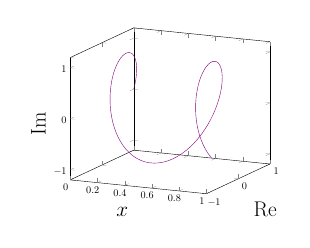
\begin{tikzpicture}[scale=0.37]
        \begin{axis}[
            view={25}{15},
            xlabel={\huge $x$},
            ylabel={\huge Re},
            zlabel={\huge Im},
        ]
          \addplot3+ [
              color=violet,
              domain=0:1,        % Changed: x from 0 to 1
              samples=100,       % Changed: more samples for smoothness
              samples y=1,
              mark=none,         % Added: removes the beads/markers
          ] (
              {x},
              {cos(deg(10*x))},  % Changed: x instead of \x, deg() for radians
              {sin(deg(10*x))}   % Changed: x instead of \x, deg() for radians
          );
      \end{axis}
    \end{tikzpicture}
    }
    \qquad
    \subfloat[Real part\label{fig:1b}]{
      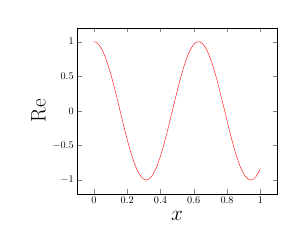
\begin{tikzpicture}[scale=0.37]
        \begin{axis}[
          xlabel={\huge $x$},
          ylabel={\huge Re},
        ]
          \addplot [
            color=red,
            domain=0:1,
            samples=100,
            mark=none,
          ] {
            cos(deg(10*x))
          };
        \end{axis}
      \end{tikzpicture}
    }
    \qquad
    \subfloat[Imaginary part\label{fig:1c}]{
      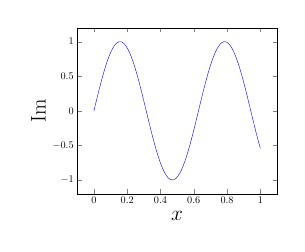
\begin{tikzpicture}[scale=0.37]
        \begin{axis}[
          xlabel={\huge $x$},
          ylabel={\huge Im}
        ]
          \addplot[
            color=blue,
            domain=0:1,
            samples=100,
            mark=none,
          ]{
            sin(deg(10*x))
          };
        \end{axis}
      \end{tikzpicture}
    }
  \label{fig:1}
  \caption{Exact solution with $k = 10$}
  \end{figure}

\end{frame}


\begin{frame}[fragile]
  \frametitle{Weak formulation (1)}

  Let's forget about our exact solution and apply conventional PDE tools,
  which are mandatory for harder problems and numerical methods. \\
  \vspace{0.6 cm}
  We will assume that $u$ is a solution and is in $H^2(]0,1[, \mathbb{C})$ (the $\mathbb{C}$ might be omitted in the next slides).\\
  \vspace{0.6 cm}
  Then, for every $v$ in $H^2(0,1)$ we multiply the equation in our domain by $\overline{v}$ and integrate over the domain, yielding:
  $$
  \int_{]0,1[}^{} u'' \overline{v} + k^2 \int_{]0,1[}^{} u \overline{v} = 0
  $$



\end{frame}


\begin{frame}[fragile]
  \frametitle{Weak formulation (2)}

  Integrating by parts, noting:\\
  $\langle u, v \rangle_{L^2} = \int_{]0,1[}^{} u \overline{v}$ (scalar product for the energy norm)\\
  and using the boundary conditions, we get:
  \begin{block}{Our weak formulation}
    \vspace{-0.6cm}
    \begin{align*}
      \forall v \in H^2(0,1), ~ k^2 \langle u, v \rangle_{L^2} - \langle u', v' \rangle_{L^2} +  ik \left[ u(1) \overline{v(1)} - \overline{v(0)} \right] &= 0
    \end{align*}
    \vspace{-0.6cm}
  \end{block}

  This is only one of the many possible weak formulations we could have obtained.
  Other choices could have been made regarding:
  \begin{itemize}
    \item The space to which $u$ belongs (test functions)
    \item The space to which $v$ belongs (weighting functions)
    \item The norm and the scalar product
  \end{itemize}


\end{frame}


\begin{frame}[fragile]
  \frametitle{Variational formulation (1)}

  We need to rewrite our weak formulation in the standardized form:
  \begin{alertblock}{A variational formulation}
    Find $u \in V_1$ such that
    \vspace{-0.3cm}
      \begin{align*}
        \forall v \in V_2, ~ a(u, v) = l(v)
      \end{align*}
      \vspace{-0.6cm}
  \end{alertblock}  
  Where:
  \begin{itemize}
    \item $V_1$ and $V_2$ are Hilbert spaces (with their respective scalar products)
    \item $a$ is sesquilinear
    \item $l$ is antilinear or linear
  \end{itemize}
  Other properties can work, but this covers most problems.
  Real-valued problems can be seen a trivial particular case.

\end{frame}


\begin{frame}[fragile]
  \frametitle{Variational formulation (2)}

  First, note that $(H^2(0,1), \langle ., . \rangle_{L^2})$ is a Hilbert space.\\
  Based on the weak formulation, we deduce our forms:
  \begin{block}{Our sesquilinear form}
  \vspace{-0.6cm}
    \begin{align*}
      a : (H^2(0,1))^2 &\longrightarrow \mathbb{C} \\
      (u, v) &\longmapsto k^2 \langle u, v \rangle_{L^2} - \langle u', v' \rangle_{L^2} +  ik \left[ u(1) \overline{v(1)} \right]
    \end{align*}
    \vspace{-0.6cm}
  \end{block}

  \begin{alertblock}{Our antilinear form}
    \vspace{-0.6cm}
      \begin{align*}
        l : H^2(0,1) &\longrightarrow \mathbb{C} \\
        v &\longmapsto ik \left[ \overline{v(0)} \right]
      \end{align*}
      \vspace{-0.6cm}
    \end{alertblock}

\end{frame}


\begin{frame}[fragile]
  \frametitle{Continuity of the sesquilinear form}
\end{frame}


\begin{frame}[fragile]
  \frametitle{Continuity of the antilinear form}
\end{frame}


\begin{frame}[fragile]
  \frametitle{Coercivity of the bilinear form}
\end{frame}


\begin{frame}[fragile]
  \frametitle{Lax-Milgram theory}

  After proving all of those properties and if $a$ was coercive,
  we could have used:
  \begin{alertblock}{The adequate complex-valued version of the Lax-Milgram theorem}
    If:
    \begin{itemize}
      \item $(V, \langle ., . \rangle_V)$ is a Hilbert space with any valid scalar produt
      \item $a: V^2 \rightarrow \mathbb{C}$ is sesquilinear (with antilinearity on the second argument)
      \item $l: V \rightarrow \mathbb{C}$ is antilinear
      \item $a$ and $l$ are continuous (let's name the constants $C_a$ and $C_l$)
      \item $\Re(a)$ is coercive (let's name the constant $\alpha$)
    \end{itemize}
    Then the problem "find $u \in V$ such that for all $v \in V$, $a(u,v)=l(v)$":
    \begin{itemize}
      \item has un unique solution $u$
      \item $\lvert \lvert u \rvert \rvert_{V} \leq \frac{1}{\alpha} \lvert \lvert l \rvert \rvert_{V'} = \frac{C_l}{\alpha}$ 
    \end{itemize}
  \end{alertblock}
  Note that other versions of the theorem exist and some properties were only chosen as conventions.

\end{frame}


\begin{frame}
  \frametitle{Fredholm theory}

  However, $a$ is not coercive

\end{frame}


\begin{frame}[fragile]
  \frametitle{Well-posedness of our problem}
\end{frame}


\begin{frame}[fragile]
  \frametitle{Galerkin equation}

  Straightforward numerical solving of the variational formulation is not possible,
  as there are infinitely many possible trial functions and weighting functions.\\
  We discretize those spaces, thus yielding:
  \begin{block}{A Galerkin equation}
    Find $u^h \in V_{1}^{h}$ such that
    \vspace{-0.3cm}
      \begin{align*}
        \forall v^h \in V_{2}^{h}, ~ a(u^h, v^h) = l(v^h)
      \end{align*}
      \vspace{-0.6cm}
  \end{block}  
  Where $V_{1}^{h} \subset V_1$ and $V_{2}^{h} \subset V_2$ are finite.\\
  Be reminded that in our case, $V_1 = V_2 = H^2(0,1)$, with the $L^2$ scalar product.\\
  One might notice that the error is orthogonal to the subspaces: 
  $$
  a(u - u^h, v^h) = a(u, v^h) - a(u^h, v^h) = f(v^h) -f(v^h) = 0
  $$
\end{frame}


\begin{frame}[fragile]
  \frametitle{Lax-Milgram Galerkin theory}
\end{frame}


\begin{frame}[fragile]
  \frametitle{Fredholm Galerkin theory}
\end{frame}


\begin{frame}[fragile]
  \frametitle{Matrix form of the Galerkin equation (1)}
  Trivial extension of Galerkine methods to complex-valued problems would be conducted by expressing functions of $V_{1}^{h}$ and $V_{2}^{h}$ as linear combinations of \alert{complex functions} (base of the discrete Hilbert spaces) with \alert{real coefficients}.\\
  \vspace{0.6 cm}
  However, for convenience, we will rather use \alert{complex coefficients} and \alert{real functions}.
  This approach is possible for complex Hilbert spaces that are complexifications of real Hilbert spaces, which is true in our case.\\
  \vspace{0.6 cm}
  The only consequence of such a choice is that we must choose the same dicretization for the real and imaginary parts of our trial and weighting functions.\\
  \vspace{0.6 cm}
  Let's note $(e_{1,i})_{i \in \llbracket 1, n \rrbracket}$ and $(e_{2,i})_{i \in \llbracket 1, m \rrbracket}$ our bases of $\Re V_1^h$ and $\Re V_2^h$.


\end{frame}


\begin{frame}[fragile]
  \frametitle{Matrix form of the Galerkin equation (2)}

  It can easily be shown that to solve the Galerkin problem, it is sufficient to test the solution over every single weighting (test) function.\\
  \vspace{0.6 cm}
  Thus, the Galerkin problem is equivalent to:\\
  Find $(u_i)_i \in \mathbb{C}^{n}$ such that:
  \vspace{-0.3 cm}
  $$
      \forall j \in \llbracket 1, m \rrbracket, ~ a \left(\sum_{i=1}^{n} u_i e_{1,i} ~ , ~ e_{2,j}\right) = l(e_{2,j})
  $$
  Note: we wrote $u^h$ in its base, i.e $u^h = \sum_{i=1}^{n} u_i e_{1,i}$.\\
  \vspace{0.6 cm}
  In our case, $a$ being linear in its first argument, the system can be written as:
  $$
  \forall j \in \llbracket 1, m \rrbracket, ~ \sum_{i=1}^{n} u_i a \left(e_{1,i} ~ , ~ e_{2,j}\right) = l(e_{2,j})
  $$

\end{frame}


\begin{frame}[fragile]
  \frametitle{Matrix form of the Galerkin equation (3)}

  Finally, the system of equations can be written as a matrix product:
  \begin{alertblock}{The matrix form of a Galerkin equation}
    Find $U \in \mathcal{M}_{n,1}(\mathbb{C})$ such that
    \vspace{-0.3cm}
      \begin{align*}
        A^{\mathsf{T}} U = L
        \vspace{-0.3 cm}
      \end{align*}

    Where:
    \begin{itemize}
      \item $\forall (i, j) \in \llbracket 1, n \rrbracket \times \llbracket 1, m \rrbracket, ~ [A]_{i,j} = a \left(e_{1,i} ~ , ~ e_{2,j}\right)$
      \item $\forall j \in \llbracket 1, m \rrbracket, ~ [L]_j = l(e_{2,j})$
    \end{itemize}
  \end{alertblock}

\end{frame}


\begin{frame}[fragile]
  \frametitle{Mesh (1)}

  The first step to finite element methods is the choice of the mesh.
  A mesh is composed of \alert{nodes} that circumscribe \alert{elements}. \\
  \vspace{0.6 cm}
  Some properties are often required for a mesh composed of closed elements $(\Omega_i)_i$ over a domain $\Omega$:
  \begin{align*}
    \bigcup_{i} \Omega_i &= \overline{\Omega} \\
    \forall i \ne j, ~ \Omega_i \cap \Omega_j &= \delta \Omega_i \cap \delta \Omega_j
  \end{align*}
  This means that nothing more but the whole domain is covered by the elements, and that elements only enventually overlap on their boundary (a hyperplane of inferior dimension).


\end{frame}


\begin{frame}[fragile]
  \frametitle{Mesh (2)}

  Mesh design is a whole discipline in itself. However, for the sake of simplicity,
  we will use a uniform mesh of element size $h$ over our unit interval.

  \begin{figure}
    \centering
    \subfloat[Iterations of a 3D mesh\label{fig:2a}]{
      \includegraphics[width=0.4\textwidth]{wrench.jpg}
    }
    \qquad
    \subfloat[1D uniform mesh (an asterisk is a node)\label{fig:2b}]{
      \pgfplotsset{width=0.4\textwidth}
      \begin{tikzpicture}
        \begin{axis}[
          xlabel={$x$}
        ]
          \addplot[
            color=blue,
            domain=0:1,
            samples=10,
            mark=asterisk,
          ]{
            0
          };
        \end{axis}
      \end{tikzpicture}
    }
  \label{fig:2}
  \end{figure}




\end{frame}


\begin{frame}
  \frametitle{Linear interpolation}

  For our 

\end{frame}



  
\section{Bibliography}
  
\begin{frame}[t,allowframebreaks]
  \frametitle{Bibliography}
  \printbibliography
\end{frame}


\section{Appendix}

\subsection{Appendix A}

\begin{frame}[fragile]
  \frametitle{Appendix A (1)}  

  We will now prove that, in order to prove that any $u^h \in V_{1}^{h}$
  is a solution of the problem for every $v^h \in V_{2}^{h}$,
  it is sufficient to show it is a solution for every base function of $V_{2}^{h}$.\\
  \vspace{0.6 cm}
  Writing $v^h$ in its basis, this can be written as:
  \begin{align*}
    \forall j \in \llbracket 1, m \rrbracket, ~ &a \left(u^h, ~ e_{2,j}\right) = l(e_{2,j}) \\
    &\Leftrightarrow \\
    \forall (v_j)_j \in \mathbb{C}^m, ~ &a \left(u^h, ~ \sum_{j=1}^{m} v_j e_{2,j}\right) = l \left(\sum_{j=1}^{m} v_j e_{2,j}\right)
  \end{align*}
  
\end{frame}

\begin{frame}[fragile]
  \frametitle{Appendix A (2)}  

  \fbox{$\Leftarrow$} Setting $(v_j)_j$ to $(1, 0, ..., 0)$, $(0, 1, 0 , ..., 0)$, ..., $(0, 0, ..., 0, 1)$ seals the deal.\\
  \vspace{0.6 cm}
  \fbox{$\Rightarrow$}
  Let $(v_j)_j \in \mathbb{C}^m$.
  $$
    a \left(u^h, ~ \sum_{j=1}^{m} v_j e_{2,j}\right) = \sum_{j=1}^{m} ~ \overline{v_j} a \left(u^h, ~ e_{2,j}\right) = \sum_{j=1}^{m} ~ \overline{v_j} l(e_{2,j}) = l \left(\sum_{j=1}^{m} v_j e_{2,j}\right)
  $$
  Respectively because $a$ is right-antilinear, the hypothesis, and $l$ is antilinear.
\end{frame}

\end{document}